\section{Scan}
\label{sec:scan}

The scan algorithm takes an array, a binary and associative operator, and an identity element.
If the operator is add, the scan algorithm computes the running sum of the input.
The identity element is 0 for addition.
As an example see \cref{tab:scan example} which shows the running sum of each element in the array.

\begin{table}[htb]
  \centering
  \begin{tabular}{r | c c c c}
    \toprule
    input & 1 & 2 & 3 & 4 \\
    operator & \multicolumn{4}{c}{$\mathtt{+}$} \\
    output (incl.) & 1 & 3 & 6 & 10 \\
    output (excl.) & 0 & 1 & 3 & 6 \\
    \bottomrule
  \end{tabular}
  \caption{Sum scan example}
  \label{tab:scan example}
\end{table}
    
A simple serial implementation is presented in \cref{lst:scan seq}.
Initially, the first element is copied to the first address of the output array, because there are no elements preceding the first element.
Next, a loop computes the running sum of the rest of the array.

\begin{lstlisting}[caption={Serial scan}, label={lst:scan seq}]
void scan(int *h_int, int *h_out, int SIZE) {
  h_out[0] = h_in[0];
  for (int l = 1; l < SIZE; ++l)
    h_out[l] = h_out[l-1] + h_in[l];
}
\end{lstlisting}

This is known as an inclusive sum scan.
Inclusive, because the given element is included in the running sum.
An exclusive sum scan results in an output where the inclusive output is shifted once to the right, and the first element is the identity element, i.e. 0 for addition.

\subsection{Hillis and Steele Scan}
\label{sec:hillis and steele scan}

For this project we work with the Hillis and Steele inclusive scan implementation.
This algorithm is performed iteratively.
Starting with step 0, on the $i$th step, each element adds itself to the neighbour $2^i$ to the left.
This algorithm is illustrated in \cref{fig:hillis steele scan}.
We have $n$ elements, and the height of the amount of steps is equal to $\mathrm{log}_2(n)$.
Thus, this algorithm runs in $\mathrm{log}_2(n)$ steps and does $n \mathrm{log}_2(n)$ amount of work.

\begin{figure}[htb]
  \centering
  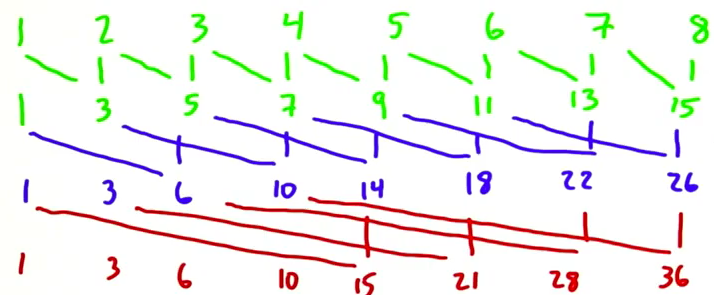
\includegraphics[width=.7\textwidth]{images/hillis-steele-scan.png}
  \caption{Hillis and Steele inclusive sum scan illustration}
  \label{fig:hillis steele scan}
\end{figure}

We present the kernel for this implementation in \cref{lst:scan par}.
Each thread calculates its position in the grid and block, and returns if it is out of bounds.
Otherwise, we make sure to add the correct element in the input or 0 if it is out of bounds.

\begin{lstlisting}[caption={Hillis and Steele scan kernel}, label={lst:scan par}]
__global__
void scan_kernel(int *d_out, int *d_in, int step, int SIZE) {
  int mid = threadIdx.x + blockDim.x * blockIdx.x;
  if (mid >= SIZE) return;

  int toAdd  = ( ((mid - step) < 0) ? 0 : d_in[mid - step] );
  d_out[mid] = d_in[mid] + toAdd;
}
\end{lstlisting}

As mentioned, this implementation is iterative and we must maintain a step variable.
For this we introduce a wrapper that handles calling the kernel with the correct values.
It is presented in \cref{lst:scan wrapper}, where the first step is 1, i.e. $2^0$.
With each iteration the step is doubled.
We copy the temporary intermediate values and make sure they are correctly updated for the next run.

\begin{lstlisting}[caption={Hillis and Steele scan kernel wrapper}, label={lst:scan wrapper}]
void scan_kernel_wrapper(int *d_out, int *d_in, int SIZE, 
                         unsigned int BYTES, int BLOCK_SIZE) {
  for (int step = 1; step < SIZE; step *= 2) {
    scan_kernel<<<GRID_SIZE,BLOCK_SIZE>>>(d_out, d_tmp, step, SIZE);
    cudaMemcpy(d_tmp, d_out, BYTES, cudaMemcpyDeviceToDevice);
  }
}
\end{lstlisting}

